\chapter{Project}\label{ch:project}

This chapter is devoted to the description of the general architectures, 
and specific algorithms.


\section{Logical architecture}

The logical architecture is composed by the following component:
\begin{itemize}
    \item \textbf{Web Service} a node that provides environment primitives to the 
        car processes (list of adjacent cars) and, at the same time, 
        can send queries to the DB component and exposes a \textbf{RESTful API}~\cite{9} 
        for the clients.
    \item \textbf{Client} a simple web page used to monitoring the simulation state
        and manage simulation settings; uses the web service APIs to render a 
        graphic interface that must be constantly synchronized (polling).
    \item \textbf{Car} a process that is the abstraction/simulation of a real car; 
        \begin{itemize}
            \item[$\rhd$] it can become a leader in order to schedule the crossing 
                order for the next turn
            \item[$\rhd$] it must check the health state and position of the other adjacent cars 
                (calls the tow truck in case of failure)
            \item[$\rhd$] it can see environment details calling a web service 
            \item[$\rhd$] it has to synchronize its local timing using Berkeley algorithm
        \end{itemize}
    \item \textbf{Distributed DBMS}, an instance of Mnesia DBMS paired 
        with the web service instance 
        (in a real distributed scenery there will be an instance of Mnesia 
        foreach web service in order to increase redundancy and robustness). 
    \item \textbf{Docker Container} wraps one or more car and/or web service instances 
        and is designed to be interconnected with all others containers 
        (using a \textbf{docker network}). 
    \end{itemize}


\section{Protocols and algorithms}

Following the \textit{divide et impera} philosophy now we are going to split the problem 
into some subproblems and solve them. 
We also provide a simplified sequence of UML (sequence) diagrams in order to 
describe the workflow/communication patterns.


\subsection{Starvation/deadlock and order method}

Ideally a car that reaches first the queue must pass before other 
incoming cars (\textbf{FIFO}).

We have to \textbf{avoid starvation} (ie. when a car waits infinite time cause the opposite queue 
has infinite length and it never has the priority) and \textbf{deadlock} (cars aren't able to 
reach the agreement). 


\subsection{Solution}

In order to avoid \textbf{starvation} in a first stage cars synchronize themselves 
(for the synchronization process we follow the \textbf{Berkeley algorithm})
in terms of local timinig and in a second stage there will be a \textbf{leader election} 
and the leader decides the crossing order. 

Using this method we also avoid 
the possibility of a \textbf{deadlock} as long as the leader is running.

In a certain instant the elected leader is the car that has reached the bridge and 
present a lower arrival time wrt. the car on the opposite side (if present); 
once the current leader crosses the bridge there is a new election.\\


\section{Synchronization problem}

Every car has a \textbf{local timing} that can \textbf{drifts} out from the 
global timing. 


\subsection{Solution}

So we need to synchronize the incoming cars using the \textbf{Berkeley algorithm}.

A new incoming car calls the \textit{environment:get$\_$adjacent$\_$cars(p)} 
method in order to get the name of the adjacent cars. 
The new car $c$ sends a message to the nearest car $n$ in order to get the current time 
(we assume that $n$ was already synchronized). 

With this information $c$ is concious of the RTT and its local drift from the global time;
so basically the global timing is the timing of the first leader. 

\begin{center}
    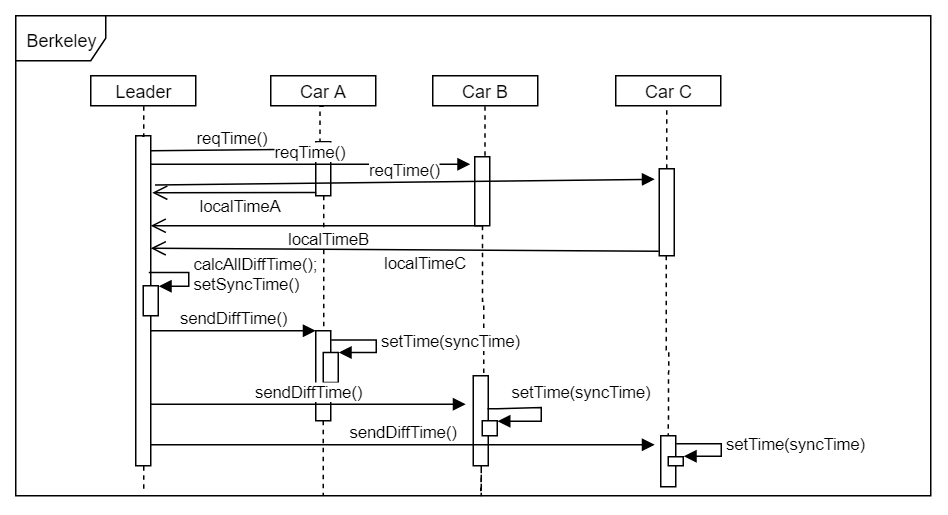
\includegraphics[scale=0.6, width=\linewidth]{assets/berkeley.png}
    \captionof{figure}{Berkeley algorithm}
\end{center}


\section{Agreement}

The current leader identifies the block of cars that will cross the bridge and notifies
this decision.  

\subsection{Solution}

Before crossing the bridge, the leader $A$ propagates a message to 
the first $n$ cars behind him (where $n$ is the capacity of the bridge). 

The message that is received 
tells them to cross the bridge if their arrival times are lower than the 
arrival time of $B$, the car on the opposite side (if present). It could be possible that only a part
of them will pass the bridge while some other have to wait for their turn.

Each car, who receives the message, checks if its arrival time is less then $B$'s: 
if so then the car can cross the bridge too, otherwise waits for its turn.\\

\noindent
The leader will always be elected by himself. Suppose that the car $A$, 
which is not a leader and hasn't the permission to cross, arrives on the bridge side.

At that point $A$ checks if there are any other car in front of her:
\begin{itemize}
\item if there is a car whose arrival time is greater then $A$'s then A 
    is the new leader;
\item if there isn't any car, A is the new leader.
\end{itemize}

\begin{center}
    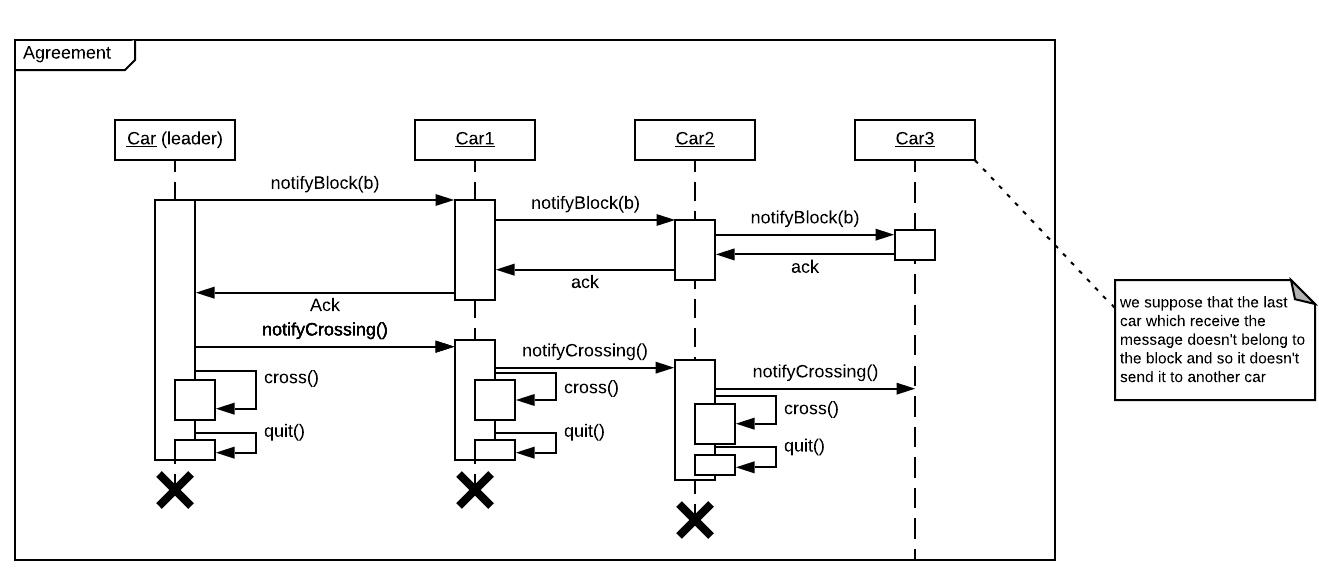
\includegraphics[scale=0.6]{assets/ds2019_3.png}
    \captionof{figure}{Agreement}
\end{center}


\section{Failures}

In case of failure, of both engine and communication system,
another car has to call a \textbf{tow truck} for help. 
If only the engine has crashed then the car
itself can call the \textbf{tow truck}.


\subsection{Solution}

Each car recursively checks if other reachable cars are safe; if a check message
hasn't any response within a certain \textbf{timeout} (depends on the $max\_RTT$ allowed) 
it is assumed that the receiver has a failure (and so the tow truck will be called). 

Once the car was removed the tow truck notifies the adjacent cars; anyway if the car
is able to send messages notifies autonomously its removal to the adjacent cars.


\begin{center}
    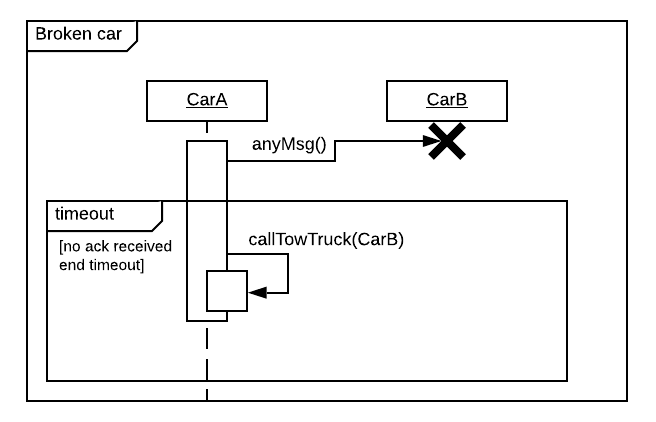
\includegraphics[scale=0.9]{assets/ds2019_4.png}
    \captionof{figure}{Car with crash type 2 (engine and system)}
\end{center}


\section{MIM attack}
\fbox{Bonus requirement, not necessary}\\

\noindent
The system must withstand a MIM attack.


\subsection{Solution}

Each message will be encrypted (HTTPS).


\section{Scalability}

The system must \textbf{scale wrt. the load} 
(the number of cars and clients can scale arbitrarily).


\subsection{Solution}

Erlang allows huge numbers of processes on the same machine so we will 
test everything locally.\\

\noindent
\fbox{Bonus requirement, not necessary}\\

\noindent
Anyway if we assume that the available machines are defined in the initialization phase,
it will be easy to rise up instances of cars and/or web services on different machines.

Can be also designed an embedded load balancer in order to avoid the web services overload 
(considering the number of calls).

\begin{center}
    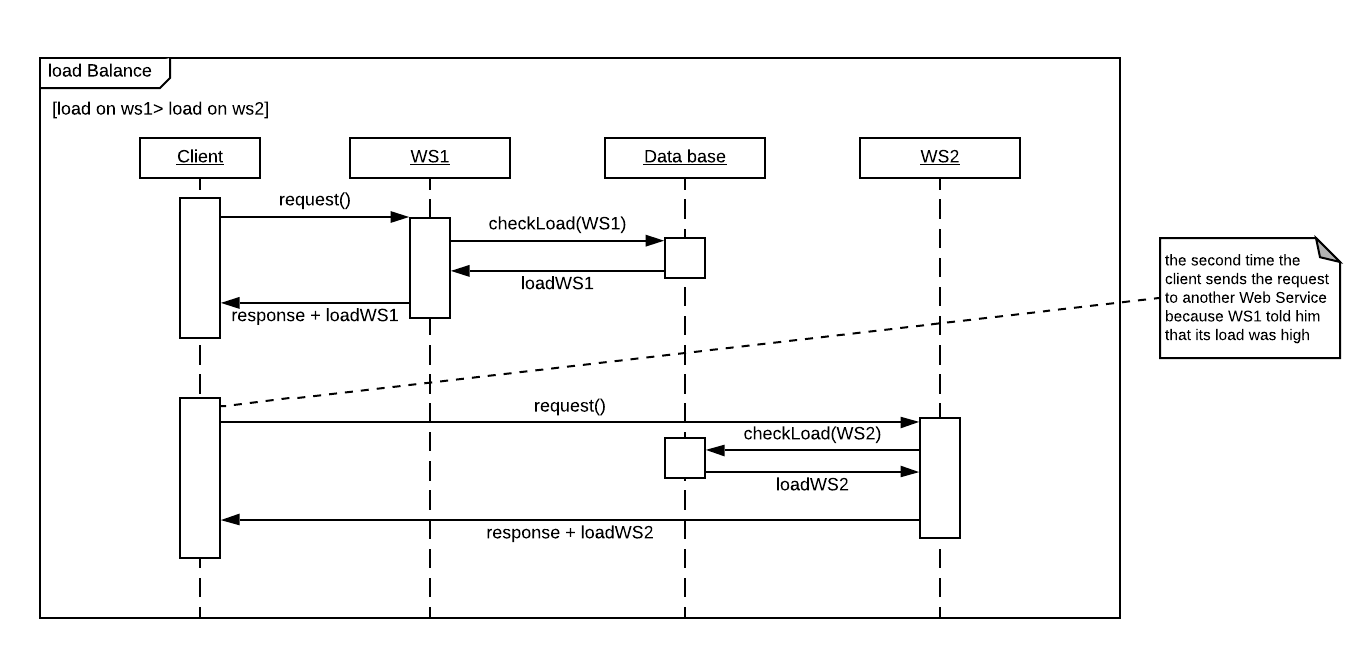
\includegraphics[scale=0.6]{assets/ds2019_2.png}
    \captionof{figure}{Load balance}
\end{center}


\section{SPOF}

The system must be resilient wrt. failures (even multiple failures);
so basically the architecture must be deeply \textbf{distributed} 
and \textbf{decentralized} (avoid any SPOF). 


\subsection{Solution}

The scalability requirement imposes that every macro-component must be scalable 
so the architecture provides a \textbf{peer-to-peer layer} of cars.

The only SPOF in this context can be the \textit{environment} component 
(which is embedded into the web services) that allows for a new spawned car to 
start a message exchange with the adjacent cars. 

This issue can be solved 
with a peer to peer layer of web services and some istances of a 
\textbf{distributed DBMS} like Mnesia~\cite{1} (but isn't a project requirement).

\begin{center}
    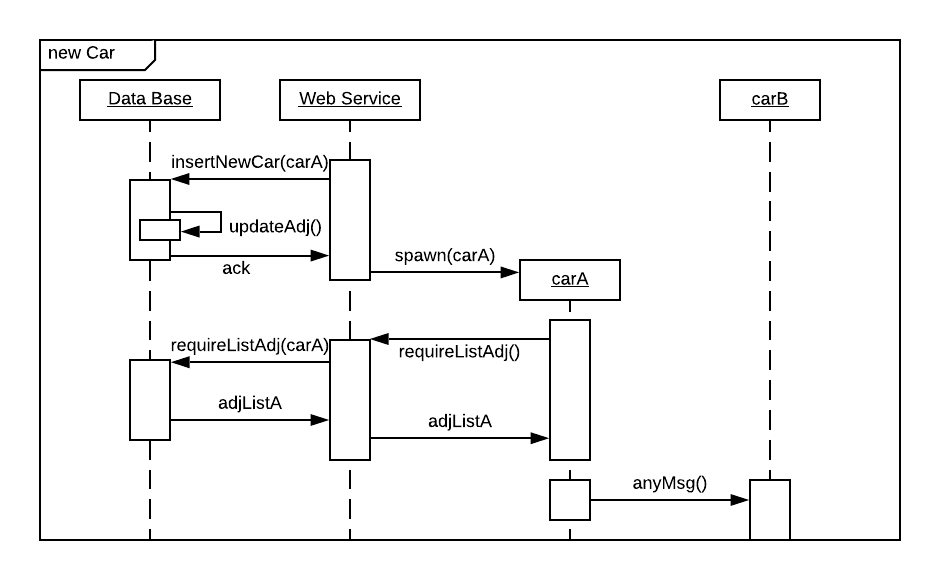
\includegraphics[scale=0.8]{assets/ds2019_1.png}
    \captionof{figure}{Creation of a new car}
\end{center}

\begin{center}
    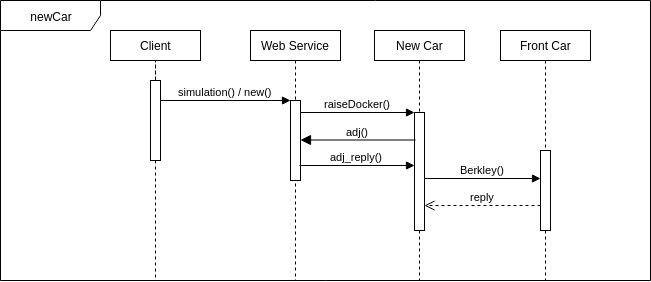
\includegraphics[scale=0.6]{assets/newCar.png}
    \captionof{figure}{Request of new car}
\end{center}



\section{Concurrency and Consistency}

Due to the asynchronicity, concurrency and time drifting is really hard 
to keep consistent the state of the cars layer with the simulation 
on the client layer. 

One way to keep an exact consistency can be to structure the algorithm on 
turns and only at the end of the turn, after the reaching of a global agreement,
launch a transactional update on the database layer. 

This way is for sure really safe but implies the implementation of some logic 
and a huge message exchange that overloads the network.

A simpler and less expensive idea (greedy) can be to leave a temporal inconsistency between 
layers state but avoid anomalous behaviours on the simulation side. \\

\noindent
Denote with $A \rightarrow B$ the order relation\footnote{
    To be precise, $\rightarrow$ is a custom order relation cause it isn't 
    reflexive (a car cannot be behind itself) and transitive but only antisymmetric.
} between two cars $A$ and $B$ that are running from left to right and $A$ 
\textbf{is immediately behind} $B$. 

So assume that in a certain instant $t_0$ 
(measured from an external and omniscient point of view) 
$A$ is in position $p_{A0}$ and B in $p_{B0}$ and 
the database layer state is consistent with the car layer state:

\begin{equation}\begin{split}
    state_{DB} = state_{Car}
\end{split}\end{equation} 

\noindent
Now before the next instant $t_1$ car $A$ moves forward of one block and car $B$
do the same after a while; we said after a while cause, as described by Lamport~\cite{Lamport:1978},
time is a continuous measure but clocks have a finite precision so 
ticks are discretizations of the time concept.\\
\indent
For this reason if we consider a turn/tick 
of one second between $t_0$ and $t_1$ we realize that in this interval some 
actions can be made so consider the case in which A and B before $t_1$ 
have sent two messages to the DB layer ($A:p_{A1}$ and $B:p_{B1}$).\\
\indent
Now from the point of view of the database layer we cannot made any assumption 
about the incoming messages cause one or both of them can be lost and/or the 
arrival order can be different from the sending order. \\
\indent
The more the third layer cannot have a consistent vision and, for example, 
can render the movement of $B$ before the transition of $A$ causing 
a visual crash (never happened).\\

\begin{tcolorbox}
\textbf{I)} Anomalous behaviours like that can easily be avoided ensuring that 
for each car must hold an order relation $\rightarrow$ and both movements 
and updates must be send respecting this relation.\\

In this way it is possible 
that the simulation renders $A$ in position $p_{A1}$ and $B$ in position 
$p_{B0}$ but this isn't a huge issue cause doesn't led to a crash so 
can be overlooked.
\end{tcolorbox}


\section{Physical architecture and deployment}

The deployment and start up consists in the following steps:
\begin{enumerate}
    \item Get the SSH credentials and IP of each computer involved in the simulation and 
        fill the \textbf{settings files} (\textit{environment.json})
    \item Launch \textit{make} and \textit{make run} commands 
    \item With a \textbf{web browser} any client can connect to the web service API and 
        manage/monitoring the \textbf{simulation state}   
\end{enumerate}

\noindent
We adopt \textbf{Git} for code versioning with a \textbf{feature-oriented} 
branching strategy with a \textbf{PR} foreach merge.

The code required for the simulation is taken directly from the project 
\textbf{repository} hosted on \textbf{GitHub}~\cite{2}.


\section{Development plan}

The proposed architecture is a \textbf{P2P} architecture flanked by a 
\textbf{client-server} architecture (\textbf{three-tier architecture}: 
client, web service and DBMS).\\

We will follow the \textbf{Agile} philosophy, splitting the development process in sprints 
of one week and adopting the \textbf{TDD}~\cite{10} methodology.
